\documentclass[a4paper,10pt,twocolumn,preprint,3p]{elsarticle}

\usepackage[latin1]{inputenc}
\usepackage{amssymb}
\usepackage{graphicx}
\usepackage{amsmath}
\usepackage{url}

\journal{Expert Systems with Applications}

\begin{document}

\begin{frontmatter}

% first the title is needed
\title{A Novel Technique for the Extraction of BYOD Security Rules Based on Genetic Programming}

\author[ugr]{Paloma De las Cuevas}
\ead{palomacd@ugr.es}
\author[ugr]{Pablo Garc\'{\i}a-S\'anchez}
\ead{pablogarcia@ugr.es}
\author[ugr]{J.J. Merelo}
\ead{jmerelo@geneura.ugr.es}
\author[isgt]{Zeineb Chelly}
\ead{zeinebchelly@yahoo.fr}

\address[ugr]{Department of Computer Architecture and Computer Technology, ETSIIT and CITIC \\
University of Granada, Granada, Spain. Tel: +34958241778. Fax: +34958248993}
\address[isgt]{LARODEC, Institut Sup\'erieur de Gestion de Tunis, Tunisia.}


\begin{abstract}
The growth in the number of personal devices in terms of variety and
computational % Does not click. Growth in the personal devices area,
              % maybe. "number" does not grow "in terms of variety". - JJ
abilities has given birth to the concept of ``Bring Your Own Device''
(BYOD), which applied to the corporate world has led companies to
create policies geared towards allowing and enabling those devices. % allowing what and enabling for what or where? Maybe allow to "carry" and enable "use as company tools"? - JJ
This allows % What is "this" here? "These policies"? - JJ
employees to bring and use their personal devices at
the company premises, on virtual private networks or otherwise while
on company work. Despite the significant advantages of this policy
such as reducing overheads and increasing work productivity, 
the
access to internal network and the assets it holds by these personal
devices, whose corporate control is forcefully limited, exposes the companies to
security threats such as leak of confidential data and access by
unauthorised users. % All this intro should be shorter and more to the
                    % point - JJ
%I have made it _larger_, better to explain concepts involved. If
%someone is able to make it shorter, please do - JJ
To handle these kinds of threats, we propose a way of detecting and controlling abnormal user
access by establishing a policy based on classification rules. Our
approach for the problem of BYOD security uses Genetic Programming
(GP) via a standard GP framework. GP is used as a promising approach % Do we prove this? - JJ
capable of performing an automatic discovery of novel and interesting
threat classification rules, with the additional feature of presenting
the new rules in an easily understandable way. % If we prove this in
                                % this paper, we should say so - JJ
The simulation results over real data and a
comparison with the results achieved by other techniques confirm the
viability, effectiveness, and applicability of the GP approach to the
BYOD security context.
\end{abstract}


\begin{keyword}
%TODO: Keywords
% Zaineb : I am proposing these keywords for now
Bring Your Own Device, Security, Genetic Programming, Rules Extraction. 
\end{keyword}

\end{frontmatter}


\section{Introduction}
\label{sec:intro}

The fast pace of new technology has led modern computing to undergo
several outstanding transitions in a short period of time. Modern
computing has moved over time to smaller, more reliable and faster
high-tech devices such as smartphones, laptops and tablets. The use of
these technologies in several forms is progressing, and has led to the
form of use known as the ``Bring Your Own Device'' (BYOD) concept or
philosophy. % Definition of the concept should have a reference too - JJ
Since its first appearance in research
\cite{ballagas2004byod} as a way to call the interaction between
people's devices and a public display, such as art or advertising, it
has become a very popular practise, integrated into companies
\cite{thomson2012byod} and even schools \cite{song2014bring}.  

In the corporate world, the BYOD
practice refers to allowing employees to use their
personal laptops, smartphones, tablets, and other mobile devices in
for work-related tasks, but not necessarily while being in the workplace This has many
advantages \cite{singh2012byod}; among them we mention saving costs --
as the company allows itself to save money on high-priced devices that
it would normally be required to purchase for their employees --, and
increasing flexibility and worker productivity as employees will not
be asked to haul around multiple devices to satisfy both their personal and
work needs, having everything they need in one device anytime and
anywhere. 
Other advantages are tied to the increase of worker satisfaction, attracting the best candidates, and the increase of engagement in the workplace and after hours \cite{singh2012byod}. 

%These advantages have made BYOD policies gain traction in the education
%sector with an increasing number of schools around the world choosing
%to implement their own BYOD policies. % reference!!! - JJ
% Also I don't see the point. Where do you want to bring this argument to? - JJ
% Ok, maybe we talk too much about BYOD at schools when we use company
% BYOD data, but it's true that schools are environments in which
% policies should be enforced too, right? Or can be applied in another
% way... So, what can we do? To create a section at the end called
% "other applications for our framework", for example? Or just mention
% it, reducing what's written now, and that's all?
% I would go for just mentioning it, because issues are much
% different. What company "assets" are we protecting here? - JJ
%In such environment, BYOD (also called Bring Your Own Technology) refers to a technology model that
%allows students to bring their own devices to school for learning in
%the classroom \cite{sangani2013byod, song2014bring}. The adoption of BYOD in schools
%is supported by the fact that technology plays a leading role in
%pupils/students' everyday lives and should, therefore, be an integral
%part of their learning. However, for most schools it is financially
%unsustainable to provide every student with the most appropriate
%up-to-date device. BYOD is therefore considered an attractive,
%cost-effective alternative, provided that many students usually own
%devices that are superior and more up-to-date than those available in
%schools. BYOD at schools has several benefits as well such as
%personalising learning experiences, encouraging students' independent
%learning, and promoting anytime, anywhere learning opportunities. % and this is important to know because... - JJ

However, there exists a big disadvantage concerning security, as
potentially unsecured devices from unaware users might interact with
important assets. Therefore, the main issue is to obtain a high level
of security, while maintining user privacy \cite{miller2012byod}.% if
                                % the issues are the same, why mention
                                % different environments separately?
                                % Besides, what assets of the learning
                                % center are you actually accessing? -
                                % JJ 
% Is this paragraph related to BYOD in schools? - JJ
Focusing on the corporate world and as previously highlighted, %my point exactly. Now you say we don't care about schools - JJ
% the BYOD paradigm has several advantages
%as it plays a leading role in increasing the
%companies benefits.  Despite of that this
%paradigm calls for a crucial need for securing company assets in the BYOD context. It is
it is clear that the uncontrolled access to internal networks by the
personal devices, for which companies have limitations in
controlling due to privacy preservation \cite{miller2012byod}, exposes the companies to security risks such as data
leakage, improper decommissioning, phishing including spear phishing, surveillance, and many
others \cite{lennon2012changing}. These threats have become the
companies main security concern, and for them it is a challenge to
assure a compromise between pushing personal devices towards
professional use and coping with their own stringent and complex
security requirements. This trend is inevitable as enterprises are
faced with questions of whether and how to manage this situation \cite{thomson2012byod}; and
thus every department must be involved in establishing security
policies and procedures to minimize the company's risks.

To this end, the Corporate Security Policies (CSPs) \cite{Kaeo:2003:DNS:1201807}, % I think a
                                % reference that defines them or to
                                % expand knowledge would be convenient
                                % here - JJ
                                % (Paloma) I added a reference but if you think it's not enough I can expand the concept
defined by the company's Chief Security Officer (CSO) are the core at the
identification of threats and the construction of a set of security rules. The description of these jobs include protecting
company assets by defining permissions to be considered for every
different action to be performed inside or outside the company's work
space, and eventually coming from the employees personal
devices. Nonetheless, CSOs build the set of CSPs based on their
expertise, and as such, they have the limitation of not knowing every
possible combination of events that might lead to a dangerous
situation. 

The aim of this paper is to propose a novel technique for extracting
BYOD security rules that help the CSO in the definition and refinement
of a set of security rules, that in the end, classify an upcoming
event or user action as permitted or not permitted.
The main idea is to create a reliable rule set
which is able to cover every new situation that may be a threat;
allowing the system to go beyond the limited set of known pre-defined
rules. In order to have the space of possible policy rules be as wide
as possible, we will need a technique that explores the rule space
efficiently and with the least assumptions about rule structure.
This is why we have decided to use Genetic Programming (GP) for dealing with the problem of
discovering novel, interesting knowledge and rules from large
amounts of data \cite{freitas2002data}, given that the up-to-date approaches are based in general pre-defined of manually defined rules \cite{ali2015analysis}. Considered part of the so-called \emph{Evolutionary
  Algorithms} \cite{back1996evolutionary}, GP are optimization
techniques inspired by natural evolution. By this method, the
solutions to a problem are internally encoded as trees, which can be
seen as a decision tree classifier \cite{safavian1990survey}. In our case, the assigned classes, or leaves of the tree, would be ``allow'' or ``deny'', acting over a certain incoming event; whilst the nodes are the conditions that have to be met to apply the action. Taking this into account, GP can be used to generate these classification trees, optimising an objective function called {\em fitness}. The fitness can be defined as the accuracy of a rule, being this the most used metric in classification \cite{witten2005data}, along with the classification error. But since there are other metrics that influence ``how good'' a rule or a set of rules is, such as the depth of the created tree or the number of nodes it has \cite{back1996evolutionary}, it would be of convenience to use them in the definition of the fitness.
Our proposed GP framework dedicated
for the BYOD context is capable of performing an automatic discovery
of classification rules, maximising the fitness, and presenting the rules in a way that is helpful for a CSO.
% Once again, there is a huge imbalance in the space and energy
% devoted to BYOD and the one you devote to GP. Except if you are
% going to publish in GPEM, which includes GP in the title, you will
% probably need to say a little bit more about GP. Even if it's GP,
% there are so many different ways of doing it that you will probably
% need to be more precise, specififying whether you mean "classic" GP
% or any other way. 
% JJ Approves this. You should say why you are using this technique as
% opposed to others - JJ

% This intro is very soft and does not have any "hard" claim. It does
% not really say what is specifically the problem we are dealing
% with, what we want to do and how it is addressing that
% problem. There should be a clear argumental line, something like 
% BYOD is very popular, but it presents security problems when you mix
% possibly compromised or unsecured devices with protected
% assets. Protecting that asset is the turf of the CSO, who defines
% security policies for asset access based on her expertise. However,
% these policies can't properly address the new threats posed by BYOD
% devices. That is why we need an automatic way of automatically
% defining these policies using known user actions and the possible
% threats they will eventually bring, especially when the action of an
% user might not result in immediate security danger, but in a
% possible future danger.
% I don't know, something like that, with more references, but with a
% clear argumental line. Without this argumental line, all the
% structure of the paper falls down in pieces. You can't create a
% proper state of the art, do the proper tests, and so on. - JJ
% This is pretty much addressed, but maybe we should have another look
% at it - JJ

The rest of the paper is organised as follows. In Section \ref{sec:SotA} we give an overview of the advances in GP applied to rule evolution and its applications; then, Section \ref{sec:problem} depicts the problem this work tries to solve, describing the available dataset and the proposed GP framework. The experimental set-up, as well as the different set of experiments that have been carried out are described in Section \ref{sec:experiments}. Section \ref{sec:gp} shows the obtained results from the application of GP to security rules extraction and, finally, the conclusions of this work along with some suggestions about how to continue our research are given in Section \ref{sec:future}.  

\section{Related Work}
\label{sec:SotA}

% (Paloma) To be extended

Since BYOD policies started to appear in companies' day-to-day policies  a lot
of research has been done about the advantages and disadvantages of
this approach \cite{singh2012byod}, as well as about how to properly implement it in order to
respect privacy while trying to secure the resources \cite{scarfo2012new, ali2015analysis, de2015corporate}.
These issues can be approached in different ways; Scarfo
differentiates in \cite{scarfo2012new} two main ones: allowing the
device to connect via desktop or application virtualisation, meaning
enough control to avoid employee's devices monitorisation; or allowing
the company to control devices
via Mobile Device Management (MDM), which has to be legally agreed
with the employee. %Mention disadvantages: the company has to provide
                   %a virtualization platform and pay for cloud
                   %resources, or the employee has to allow the
                   %company to control its own device, which
                   %eventually dispels two of the advantages of BYOD
                   %policies: low overhead cost and preservation of
                   %privacy. (something like that). 
 Ali et al. expand from Scarfo's study in
\cite{ali2015analysis} reviewing both BYOD access control
 and security models. The authors further distinguish
between MDM and Kernel Modifications inside the security models, and
conclude with the description of a proposed model which combines most
of the reviewed solutions, i.e. MDM and Virtual Private Network (VPN)
access together with an encrypted container for the accessed
information depending on the level of restriction. However, from all
the papers in \cite{ali2015analysis} claimed to enforce policies, only
in \cite{rhee2013high} the authors actually describe how the policies
are enforced by describing which data is monitored. In any case, none
of the papers mention the application of GP to the enforcement of the
security policies, but other techniques such as the implementation of
blacklists to avoid the installation of forbidden applications, or
whitelists to allow only certain ones. These techniques can be useful
with respect to the implementation of already defined security
policies, but our method allows to discover new security policies,
which in the case of black and white lists, can evolve them to include
new and/or malicious applications. 
 %Pablo: If previous papers describe some computational methods I would add to the last paragraph some of the techniques used. "...security policies, but other techniques such as ... These techniques can be useful with respect to... but our method is awesome because...".
 % (Paloma) I've included more information, please ckeck :D

Research in BYOD has been accompanied by innovation in products released
to help companies implement or streamline the process of adoption of the BYOD
concept. In \cite{de2015corporate} there is a description of the
market solutions that the main manufacturers have developed to such
purpose. The level of security and privacy preservation offered by
these applications is different depending on the solution. % A SOA
                                % section establishes the state of the
                                % art, it's not a catalogue. As well
                                % as above, here you would have to say
                                % what is the disadvantage of these
                                % approaches and why you are going to
                                % do it better than them.
                                % (Paloma) Fixed this with:
None of the reviewed solutions, but one, seem to offer a dynamic creation of rules in the database used for incident detection. The one called MUSES does implement rule inference and mentions the use of GP to perform this task. In this work we extend the description of the rule inference process, as well as the details of its implementation and the results after applying it to the data gathered with the very same MUSES application (see Section \ref{subsec:data}).

%Non sequitur. What do you mean here? Why are you talking about this
%here? Extracted data from what? Start with something like "Previous
%papers have commented on the issue of using quality data to extract
%rules from that that are general and accurate..." - JJ
% (Paloma) Done
Previous papers have commented on the issue of using quality data to obtain accurate and valuable extracted knowledge, which is specially difficult when dealing with datasets taken from real world problems, where the sensors cannot work properly at a certain time. % or the data can present imbalance.
To avoid this, researchers have advanced the state of the art in the precision of the
devices. For instance, in \cite{rios2015mobile}, the authors focus on
the importance of having an accurate measure of the location of the
devices. Although their approach seems to encroach upon employees'
privacy, they implemented a mobile information system for BYOD
adaptation and tested it in both Android and iOS devices. The authors
concluded that the efficiency of their system, along with the
possibilities of the hardware in the devices, results in a location
error of less than 50 meters with a 95\% confidence level. These
promising results allow the companies to use the location of their
employees to apply certain security policies.

%Another barrier to obtain good quality knowledge discovering are datasets that present imbalance, because they normally bias the elaboration of classification rules or trees towards the majority class - the class with higher representation in the dataset - \cite{japkowicz2002class}. In this sense, solutions can be found in literature in order to reduce the bias while performing classification tasks, such as in \cite{chawla2005data} and \cite{sun2009classification}. However, as we have center our proposal in GP, we have studied Bhowan et al.'s work in \cite{bhowan2012developing}, where they present a comparison between many different types of fitness functions, testing on various unbalanced datasets, with different minority-class/majority-class ratios.

Even when a lot has been advanced in preprocessing techniques in order to work with quality and accurate data \cite{han2011data}, still there is room for research in the discovery of new rules from real world data. To the best of our knowledge, there is no tool that helps CSOs in
developing new security rules via GP, % But this is a very hard
                                % claim. It should go to the
                                % introduction!!! - JJ
                                % (Paloma) Will study this)
 even as this method has been
indeed applied to classification -- from which classification rules
can be obtained -- , as described by Espejo et al. in
\cite{espejo2010survey}. Their work theoretically supports our
decision of applying GP to obtain security rules in a BYOD
environment. Furthermore, the works they review have applications in
all fields but not exactly the one we focus on here. The authors
studied three papers which use GP for classification with
communications data, but mainly for intrusion detection and e-mail
spamming. Also, in \cite{DeFalco2002257}, a system which discovers
rules for the PROBEN1 databases via GP is described. As happened in
the survey of Espejo et al., from the six databases inside PROBEN1 and
analysed by these authors, none is related to security. In
\cite{Tsakonas2004195} the authors also extract rules with \textsc{IF
  \ldots THEN} structure through GP, although for medical purposes. Futhermore, Alex A. Freitas deeply studied the application of GP to Data Mining (DM) in \cite{freitas2002data}, providing the necessary knowledge and guidelines to design a GP framework for DM applications. Section \ref{subsec:solution} will describe in detail which solution has been built from what has been found in the work of Freitas.
%Pablo: link previous paragraph with next one. Also, I would not use "on the other hand" below as it is not clear which is the "first hand". For example: "... rules via GP, even as this method has been applied to classification..."
% (Paloma) Done, check please!

%Once again, this paragraph does not follow the previous one. Maybe
%move it one paragraph up, where you are talking about proper training
%data. 
The lack of BYOD-related security databases is a hindrance for the
proliferation of research in this field. As seen, there actually exist
a number of datasets related to malware, e-mail spamming, or URL
requests \footnote{http://www.secrepo.com/}, but none about the use
that people make of their smartphones. This situation clearly exists
due to privacy considerations. Miller et al. \cite{Miller201253}
firmly state that the issue of privacy is even more important than the
security issue, although it does not receive the same
attention. Furthermore, when the MDM solution is described in
\cite{ali2015analysis}, the authors mention the privacy concerns the
employees may have due to the processing that the company makes over
all their behavioural data. And even after anonymising the resulting
dataset, one can still, in certain cases, identify a user of the
company the data comes from by processing the data. If this principle
cannot be guaranteed, the data should not be released
\cite{boillat2014handbook}. 
% TODO Pablo: I would explain here again the issue adding "This is the
% reason we can not release the dataset used in the experimental
% section, because our data includes..." BUT if we release it (issue
% #20), we can say that we are awesome and cool researchers by doing
% it 
% (Paloma) Ok then I leave this as TODO once we decide if we can
% release it.
% I think there's no problem with releasing it, but maybe you should
% ask Anna. - JJ

%Pablo: move this paragraph after the market product analysis. So, the
%SOA outline should be: 1) BYOD is a thing 2) There are some stuff
%done (market product, extracted data...) 3) However, in previous
%works there are stuff that SHOULD be done (GP and releasing datasets)
%for some fancy reasons, and 4) In this paper we do this and that to
%solve it. 
% Missing is "there is some trouble on finding data", but if we are
% not releasing this, maybe we should just be quiet about this - JJ
% (Paloma) Re-organised, I think well, but check in case I didn't move it to where you suggested.

\section{Problem Description}
\label{sec:problem}

As previously highlighted, the main idea behind the corporate security policies, which are defined by the CSO, is to build a basic, fixed, and well defined set of rules. These rules have the form of \textsc{IF \ldots THEN} clauses,  and by them the company system allows or denies access to the company assets, which can be seen as the actions being classified as allowed or denied. In this sense and while facing a security breach from a BYOD system, the set of rules will be tested looking for a matching between the access' characteristics and the rules' premises -- the conditions expressed in the IF part, also known as the description of the rule \cite{DeFalco2002257}. If a matching is found then the decision can be made, by checking the conclusion part of the rule, which comes after the THEN and indicates the class \cite{DeFalco2002257}, either by allowing or denying employees' access to non-confident or non-certified data, for example. However, it is important to mention that the companies' security rule set defined by the CSO is based on known and previously recognised accesses and thus it cannot cover the whole possibly safe and risky search spaces. Therefore, there is an urgent need to develop a system capable of discovering a more reliable rule set which should be able to cover every new situation that may be a threat. Hence, allowing the company security system to go beyond the limited set of known, pre-defined rules.

Our proposed solution is based on a novel GP framework dedicated for the BYOD context capable of performing an automatic and wider discovery of classification rules. More precisely, our GP based framework will, first, extract all the possible values of every attribute in the data at hand and then make the ``RuleGeneticAlgorithm'' evolving. % (Paloma) Pablo, more fancy way of saying this?
Specifically, in this context, we have decided to follow the more conventional approach in Genetic Algorithms, the Pittsburgh approach \cite{freitas2002data}, meaning that each individual is seen as a set of rules. The best individual is thus the set which rules covers the maximum patterns. The last step would be to present the rules to the CSO of the company and tune the algorithm according to the decision of finally including or not the set of rules in the main security policy. The description of the used data and further explicit details about our proposed solution are given in what is next.

\subsection{Available Data}
\label{subsec:data}

Anonymised user data has been used to perform the experiments for this work. The set of data has been gathered from the trials that were performed during the development of an FP7 European Project, called MUSES \cite{DBLP:conf/sac/MoraCGZJEBAH14}. In these trials, a group of users tested a smartphone and PC application meant for securing a BYOD environment. The application generates warnings when the users acts in a dangerous way. Technically, these warnings are triggered by a set of initial and pre-defined rules, so that when certain conditions are met in an ``event'' (an action performed by a user), the corresponding action could be allowed - nothing happened - or denied, where a warning appears.

The dataset contains, thus, a set of these ``events'' from which a number of attributes (variables) have been extracted or are given by the application itself. The attributes can be classified in different ways, one of them is based on whether they are directly read from the application or inferred after processing the read data. Therefore, we distinguish between:
\begin{itemize}
  \item Attributes given by the tested application: these attributes are related to the type of the event (action), its timestamp, or the application which originated the event, among others.
  \item Attributes inferred from the information in the database: the information given by the aforementioned attributes, along with the rest of information already existing in the database, helps inferring other attibutes.
      % (Zaineb) This sentence is weird. Please clarify it Paloma. I did not get what you mean here.
      % (Paloma) I hope it's more clear now
       These are, for instance: all extra information related to the origin, like the user position in the company or the device Operating System; the configuration of the device, such as WiFi or Bluetooth being enabled; and even lexical properties of the user password, in order to avoid storing the password itself or using it for classification or rule generation.
\end{itemize}

The trials had a duration of a month plus a week, and a total of 153270 events were registered in the database. It is important to note that from all of those events, almost 65\% were not useful for knowledge extraction purposes, as they were events of \textit{log in}, \textit{log out}, or \textit{restarting the server}. The other 35\% (53296 instances) were considered as \textit{important} because they did contain information about user actions such as opening files or sending emails in a certain connection environment, changing security properties, or installing apps. Altogether, there are 38 attributes plus the class, which can take two possible values: GRANTED or STRONGDENY.

With respect to the balance between the classes, the dataset is unbalanced with the following ratio: 49289 instances are labelled as GRANTED and 4007 are labelled as STRONGDENY.

\subsection{Proposed Solution}
\label{subsec:solution}
% (zaineb) I prefer adding a sentence here as an introduction. What do you think Paloma?
% (Paloma) I agree, but as Pablo didn't finish the section, I prefer to wait :)
% (Paloma) I added the introduction sentence! What do you think?
As previously highlighted, in this work we propose a system which is able to process a set of user actions that have been allowed or denied based on initial, simple rules, and discover new rules by exploring the whole space of possible combinations among the attribute values. The proposed method uses GP to create a tree to model the different rules, given that the problem can be seen as a classification one and therefore the model can be a decision tree \cite{safavian1990survey}. Then, the generated tree is a binary tree of expressions formed by two different types of nodes:

\begin{itemize}
\item {\em Variable}: it is a logical expression formed by a name, an operator and a value. It is the equivalent to a ``primitive'' in the field of GP \cite{back1996evolutionary}.  \\
    Examples:
   \begin{math}
     \left \{
   \begin{array}{l}
     \texttt{password\_length<5} \\
     or \\
      \texttt{event\_level=>COMPLEX\_EVENT}
   \end{array}
   \right .
   \end{math}
\item {\em Action}: it is a leaf of the   tree and therefore, a ``terminal'' state. Each decision is the result of applying the rule, so it is limited to two terms which are \texttt{GRANTED} or \texttt{STRONGDENY}.
\end{itemize}

At the same time, the variables can be differentiated into three types, described as follows \cite{witten2005data}:

\begin{itemize}
\item {\em Binary Variable}: those with a boolean value, for instance, variables that are related with the device services switched on or off and important features such as the device having or not an antivirus installed.
\item {\em Categorical Variable}: the ones with nominal values, where it is defined a list with the possible values it may have, in order to randomly pick up one in the creation of the rules.
\item {\em Numerical Variable}: those with a numerical value, for which both maximum and minimum values are specified.

\end{itemize}

The tree is translated to a set of rules starting from the leafs to the root node passing each time by the ancestors. An example of a rule can be presented as follows:
%TODO Show this more fancy :P (Pablo)
% (Paloma) I've shortened the rule a bit for the sake of clarity 

\begin{verbatim}
device_has_antivirus=false AND
password_length<5 AND
user_role=>Administration OR
device_is_rooted=true THEN=STRONGDENY
\end{verbatim}

Rules presented in this way offer good readability which is key to understand the relation between the attributes and how the described situation may, or may not, be dangerous. In the example, the system would have inferred that an action from a device without antivirus, a short password, and rooted or belonging to an administration employee, should be denied.
% (Paloma) Shall we explain what a rooted device is?

With regard to the fitness, in the application of GP to classification the most used metric to calculate it is the accuracy \cite{espejo2010survey}. The accuracy is normally obtained as the ratio of the correctly classified instances among the total of instances. To this end, in \cite{witten2005data} the authors use the concepts of true positive/negative and false positive/negative. The first refer to the instances classified correctly, and the latter are those instances that should be negative (positive) but are classified as positive (negative), therefore they are false positives (negatives). Using this nomenclature, a Fitness defined as the accuracy or \textit{coverage} would be expressed as follows:

% Saving this for later \cite{DeFalco2002257}

\begin{equation}
\label{eq:coverage}
f_{c} = TP + TN - (FP + FN)
\end{equation}

This kind of Fitness is used in maximisation problems, given that the ideal value of $f_{c}$ is the whole training dataset, $S_{tr}$. Additionally, to take into account the simplicity of the individuals, either they are a rule or a set of rules, in \cite{witten2005data} they introduce a measure of the generated trees complexity by this expression:

\begin{equation}
f_{s} = N_{nodes} + depth
\end{equation}

So that combining $f_{c}$, $f_{s}$ and introducing an $\alpha$ variable inside [0, 1] to tune up the degree of allowed complexity, the problem becomes now a matter of minimising this formula:

\begin{equation}
\label{eq:complexFitness}
Fitness F = (S_{tr} - f_{c}) + \alpha f_{s}
\end{equation}

\section{Experiments Description}
\label{sec:experiments}

Sub-tree crossover and 1-node mutation evolutionary operators have been used, following our previous works that have used these operators obtaining good results \cite{EvoStar2014:GPBot}. In this case, the mutation randomly changes the complete variable of a node or mutate the complete value. Each configuration is executed 30 times, with a population of 32 individuals and a 2-tournament selector for a pool of 16 parents.


Table \ref{tab:parameters} summarizes all the parameters used.

\begin{table}
\begin{center}
\begin{tabular}{|c|c|}
\hline
{\em Parameter Name} & {\em Value} \\\hline
Population size & 32 \\\hline
Crossover type & Sub-tree crossover \\ \hline
Crossover rate & 0.5\\ \hline
Mutation  & 1-node mutation\\ \hline
Mutation step-size & 0.25 \\ \hline
Selection & 2-tournament \\ \hline
Replacement & Generational with elitism\\ \hline
Stop criterion & 50 generations \\ \hline
Maximum Tree Depth & 10 \\ \hline %PABLO: CONFIRM THIS!
Runs per configuration & 30 \\ \hline
\end{tabular}
\caption{Parameters used in the experiments.}
\label{tab:parameters}
\end{center}
\end{table}

The used framework is OSGiLiath, a service-oriented evolutionary
framework \cite{DBLP:journals/soco/Garcia-SanchezGCAG13}. The
generated tree is converted to...
%Please remenber to finish this - JJ

All the source code used in this
work is available under a LGPL V3 License in
\url{http://www.osgiliath.org}. 

%\subsection{Results from Classifiers}
%\label{subsec:classifiers}

%\subsection{Results from Association Algorithms}
%\label{subsec:association}

%\subsection{Results from Clustering}
%\label{subsec:clustering}

%\subsection{Results from Genetic Programming}
%\label{subsec:gp}

%\section{Discussion}
%\label{sec:discussion}

\section{Results from Genetic Programming application}
\label{sec:gp}

\begin{figure*}[h!tb]
\centering
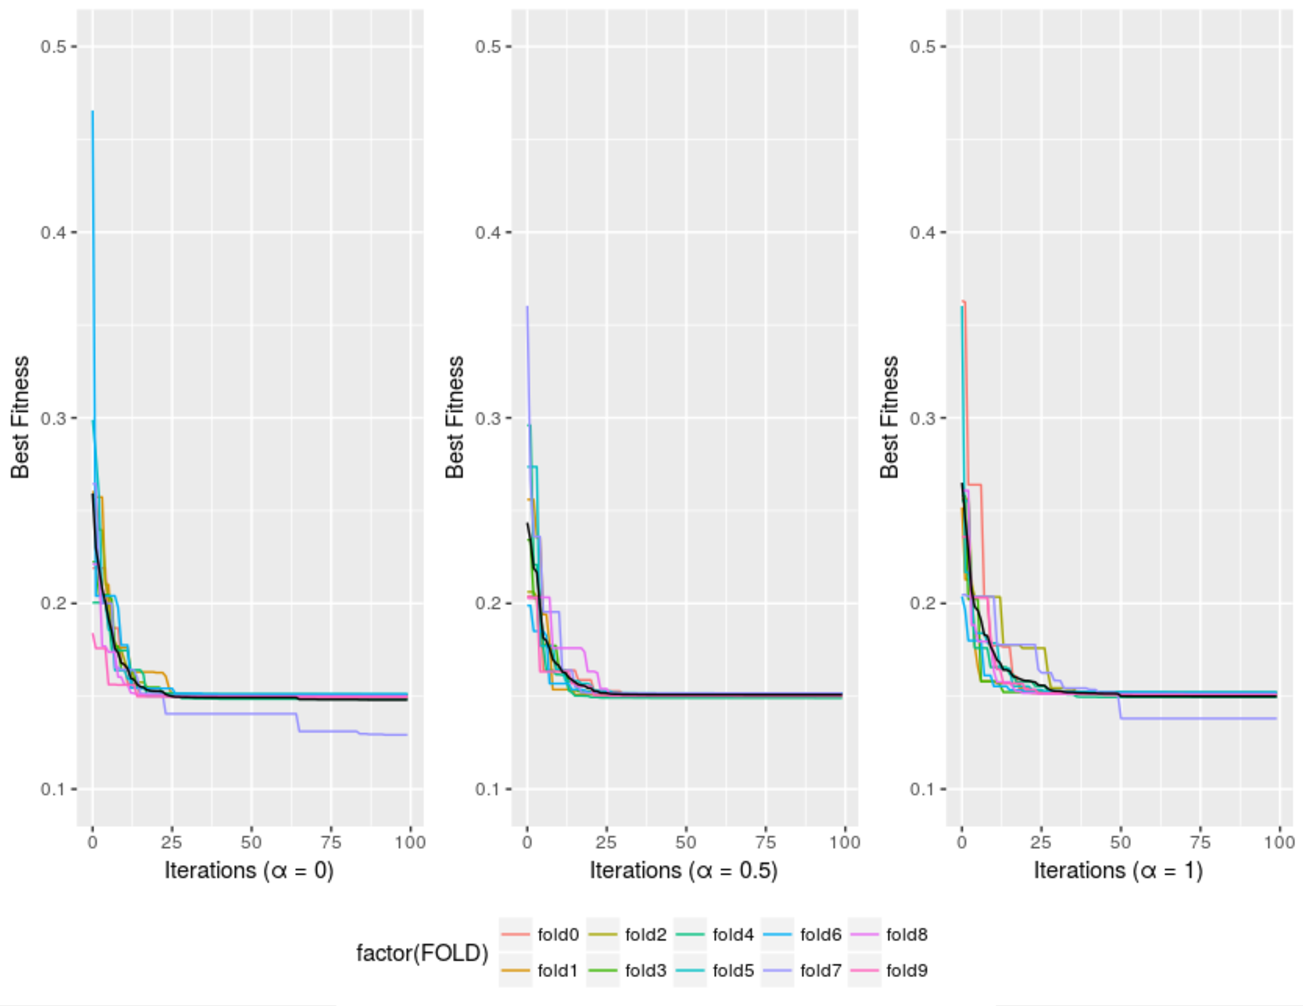
\includegraphics[width=\textwidth]{img/tree_ind_diff_alpha.pdf}
\caption{Best Fitness, calculated from Equation \ref{eq:complexFitness}, obtained for every fold or data partition, and for three different values of $\alpha$.}
\label{fig:tree_ind_diff_alpha}
\end{figure*}

\begin{figure*}[h!tb]
\centering
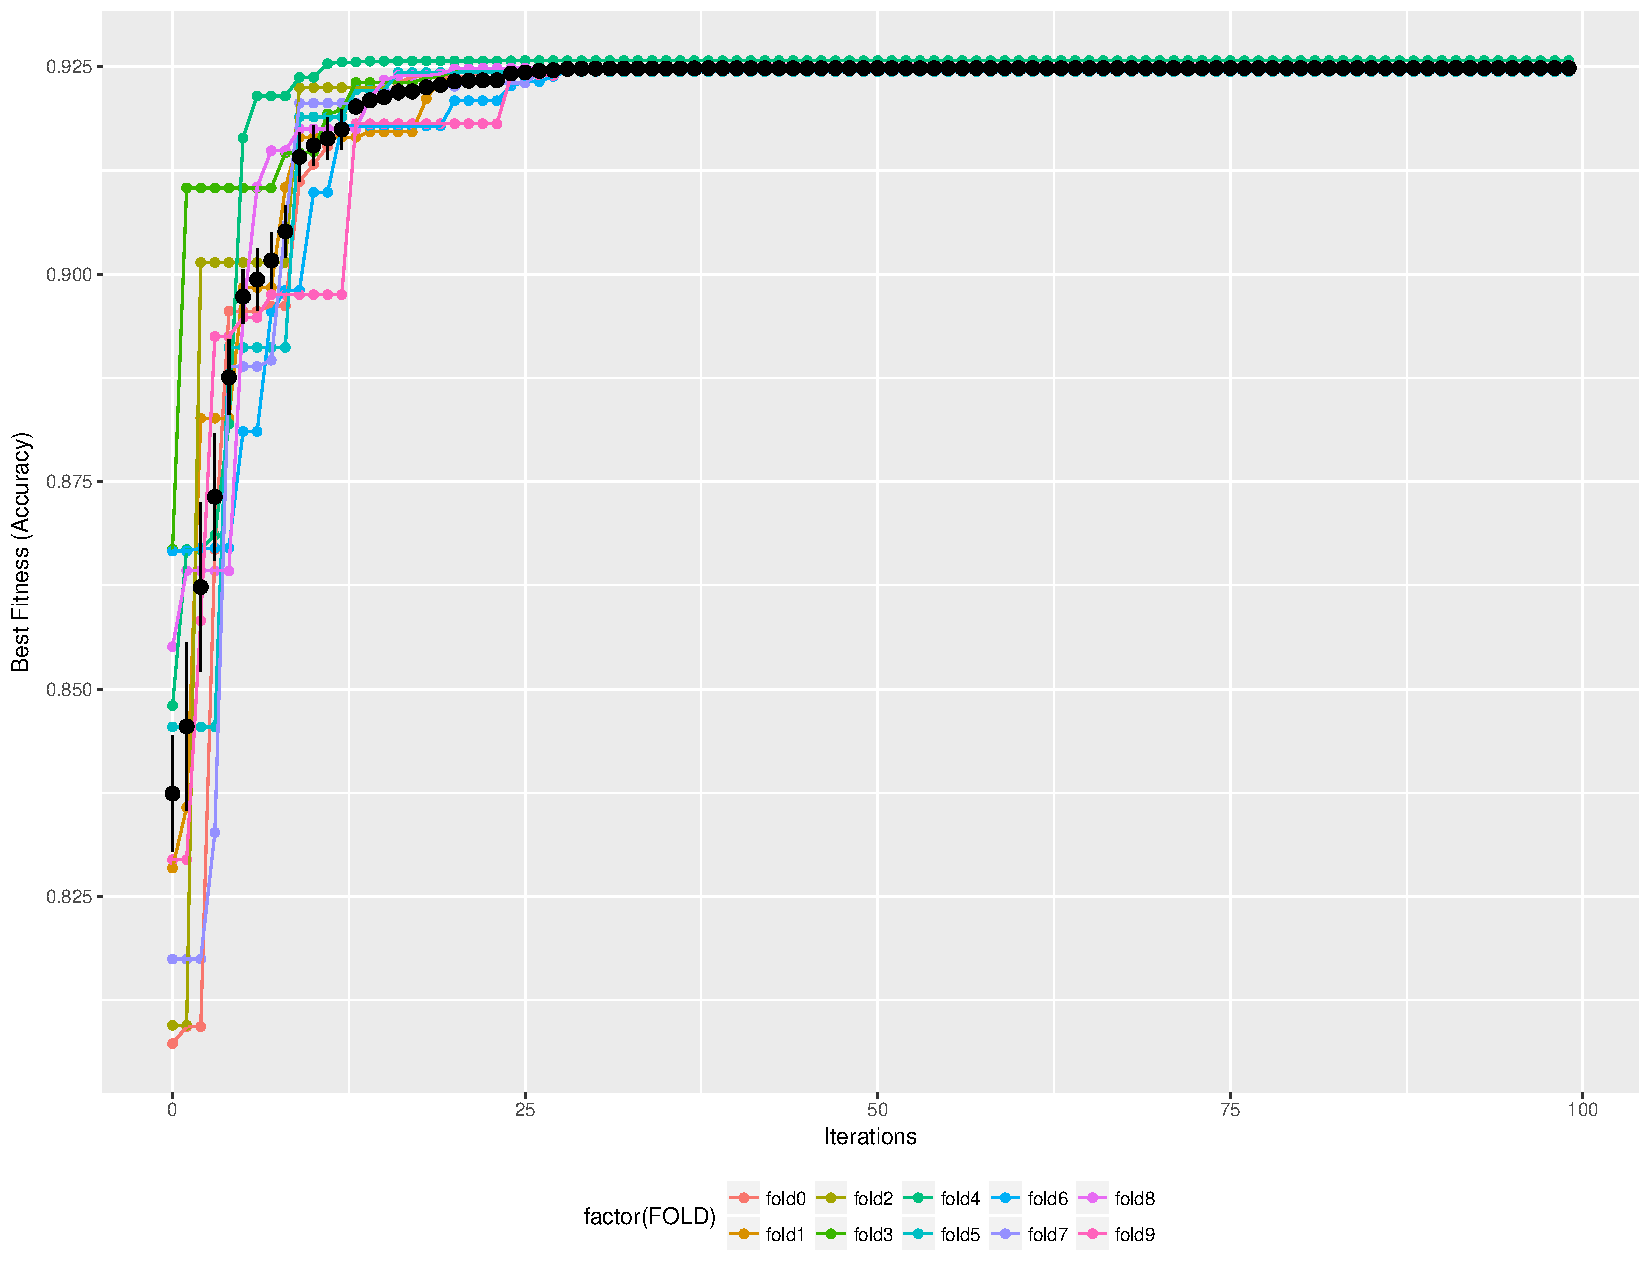
\includegraphics[width=\textwidth]{img/tree_ind_coverage.pdf}
\caption{Best Fitness, calculated from Equation \ref{eq:coverage}, obtained for every fold or data partition.}
\label{fig:tree_ind_coverage}
\end{figure*}

\begin{figure*}[h!tb]
\centering
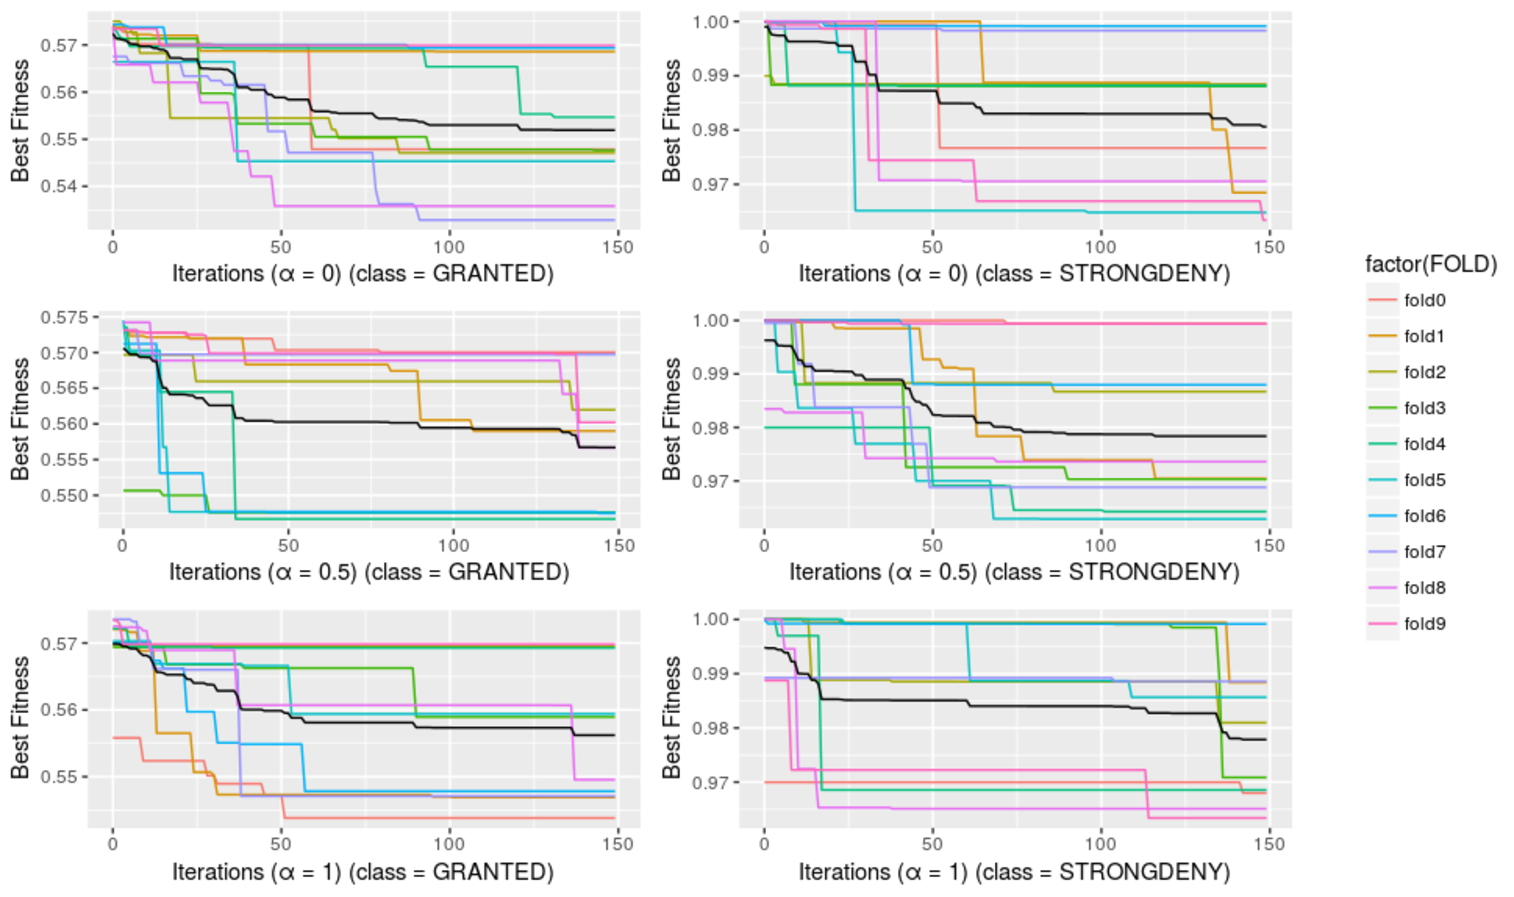
\includegraphics[width=\textwidth]{img/list_ind_diff_alpha.pdf}
\caption{Best Fitness, calculated from Equation \ref{eq:complexFitness}, obtained for every fold or data partition, and for three different values of $\alpha$.}
\label{fig:list_ind_diff_alpha}
\end{figure*}

\begin{figure*}[h!tb]
\centering
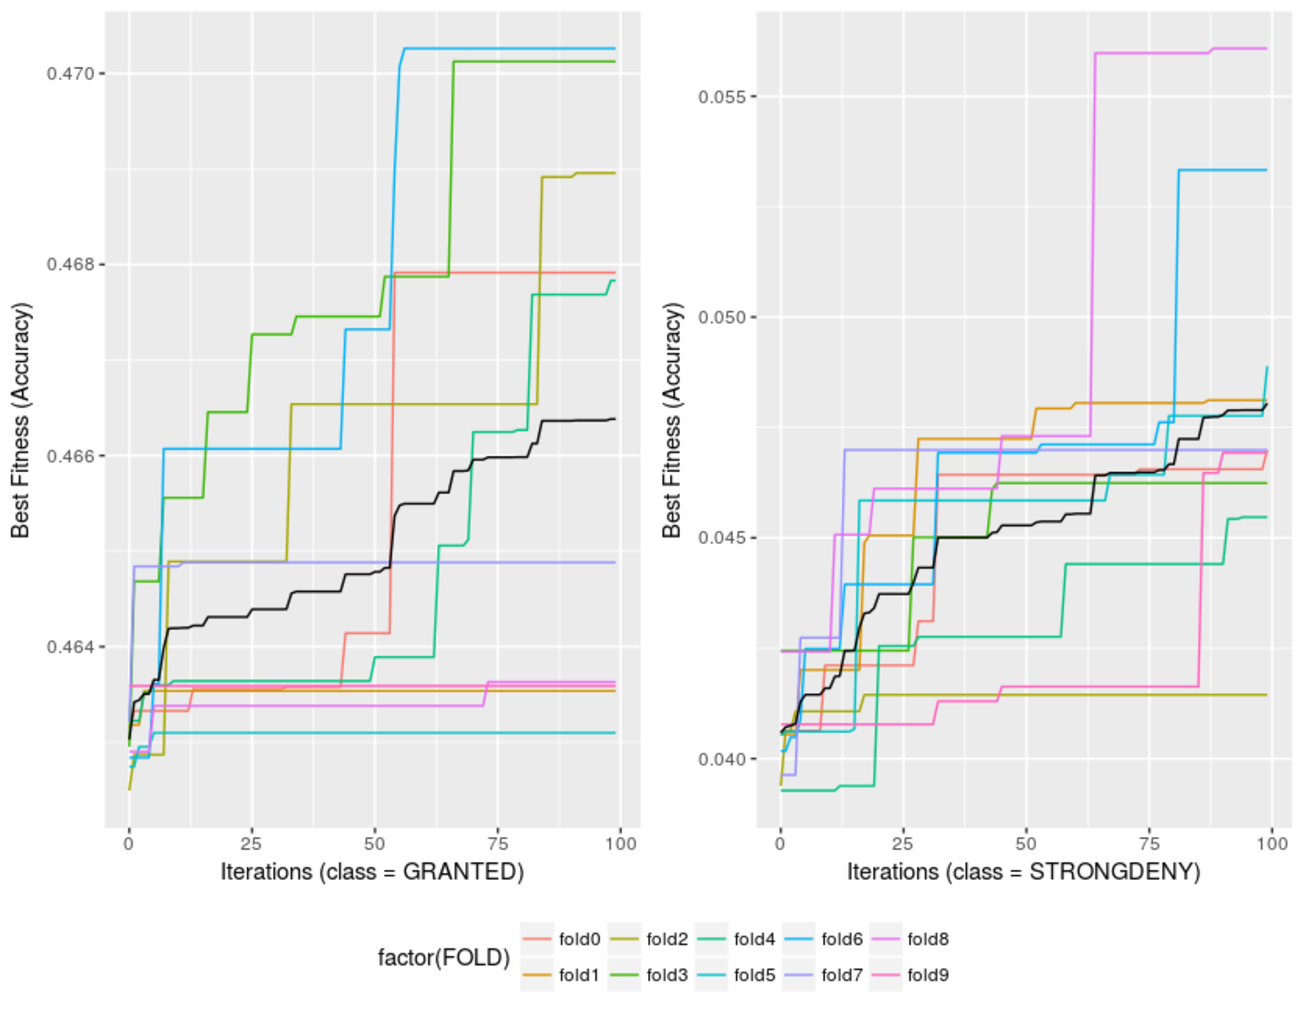
\includegraphics[width=\textwidth]{img/list_ind_coverage.pdf}
\caption{Best Fitness, calculated from Equation \ref{eq:coverage}, obtained for every fold or data partition.}
\label{fig:list_ind_coverage}
\end{figure*}


\section{Conclusions and Future Work}
\label{sec:future}

\section*{Acknowledgments.}

This work has been supported in part by TIN2014-56494-C4-3-P (Spanish
Ministry of Economy and Competitivity), PROY-PP2015-06 (Plan Propio
2015 UGR).

\bibliographystyle{elsarticle-num}
\bibliography{GPrules,geneura}

\end{document}
